\documentclass{article}
\usepackage{url}
\usepackage{graphicx}
\usepackage{subcaption}
\usepackage{float}
\graphicspath{ {./Immagini/} }

\begin{document}

\title{Relazione Progetto Big Data e Business Intelligence}
\author{Ferrara Luca  Matricola: 312173}
\maketitle
\pagebreak
\tableofcontents
\pagebreak
\section{Introduzione}
Il progetto assegnato prevede di gestire un modello di Machine Learning per fare un task di classificazione relativo al dataset: \url{https://www.kaggle.com/datasets/jimschacko/airlines-dataset-to-predict-a-delay}; \\
Il dataset riguarda un numero di voli americani e il task è di predirre se il volo avrà un ritardo o no.  Ecco come è composto il dataset:
\subsection{Dataset}
Il dataset è composto da 8 feature e 539383 instanze:
\begin{itemize}
\item id \\
Feature non utile che verrà rimossa, identificativo per il volo;
\item Airline \\
Indica la compagnia aerea;
\item Flight \\
Indica il tipo di volo;
\item AirportFrom \\
Indica l'aeroporto da dove parte il volo;
\item AirportTo \\
Indica l'aeroporto dove atterra il volo;
\item DayOfWeek \\
Giorno della settimana;
\item Time \\
Tempo del volo;
\item Length \\
Lunghezza del volo;
\item Delay \\
Indica se il volo è in ritardo (0 no, 1 si);
\end{itemize}
\section{Data Visualization}
\begin{figure}[H]
  \centering
  \begin{subfigure}[b]{0.4\linewidth}
    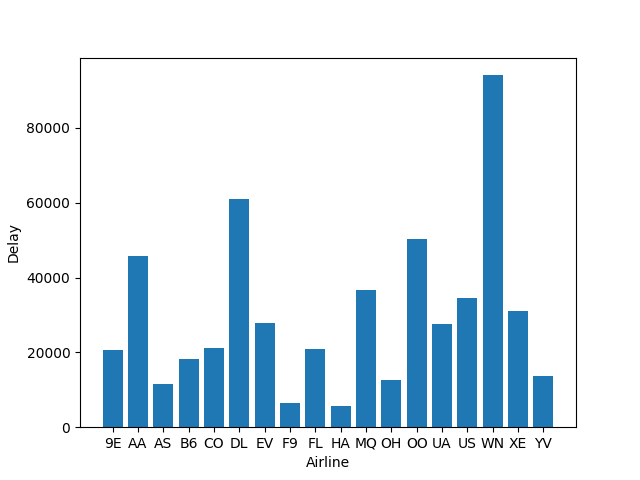
\includegraphics[width=\linewidth]{AirlineDelayCorrelation}
     \caption{Correlazione tra Volo e Delay}
  \end{subfigure}
  \begin{subfigure}[b]{0.4\linewidth}
    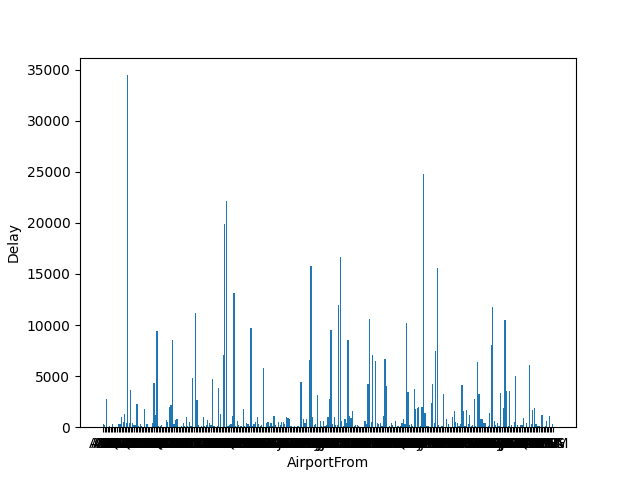
\includegraphics[width=\linewidth]{AirportFromDelayCorrelation}
    \caption{Correlazione tra Origine e Delay}
  \end{subfigure}
  \begin{subfigure}[b]{0.4\linewidth}
    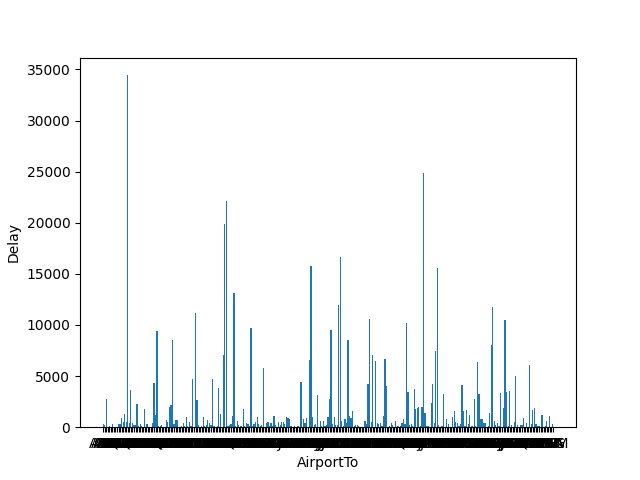
\includegraphics[width=\linewidth]{AirportToDelayCorrelation}
    \caption{Correlazione tra Destinazione e Delay}
  \end{subfigure}
  \begin{subfigure}[b]{0.4\linewidth}
    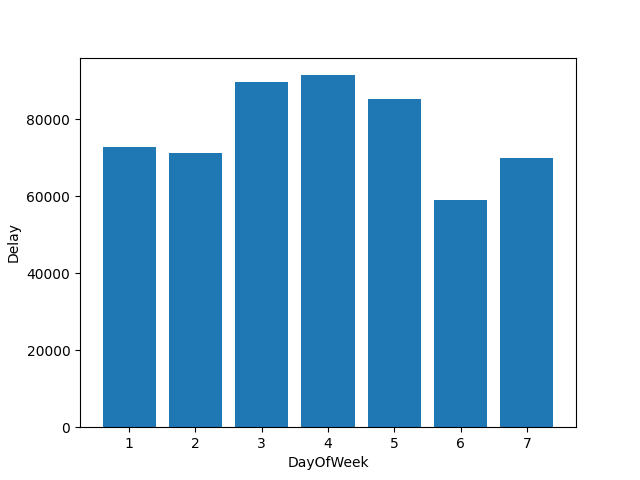
\includegraphics[width=\linewidth]{DayOfWeekDelayCorrelation}
     \caption{Correlazione tra Giorno della Settimana e Delay}
  \end{subfigure}
  \begin{subfigure}[b]{0.4\linewidth}
    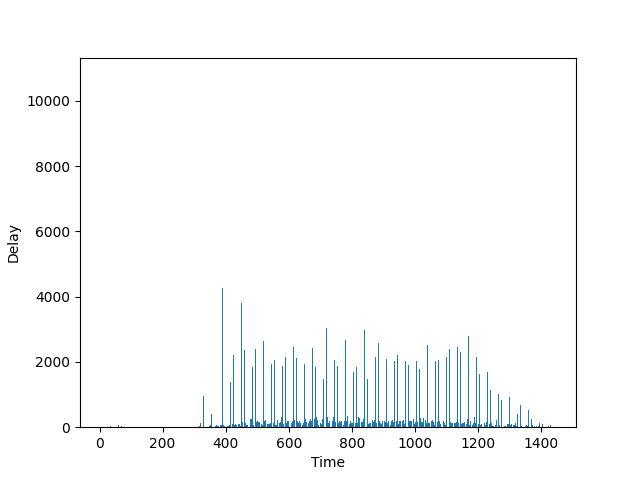
\includegraphics[width=\linewidth]{TimeDelayCorrelation}
    \caption{Correlazione tra Tempo di Volo e Delay}
  \end{subfigure}
  \begin{subfigure}[b]{0.4\linewidth}
    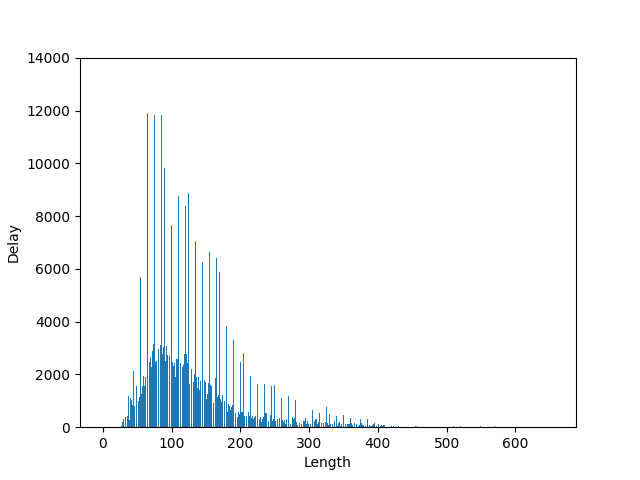
\includegraphics[width=\linewidth]{DistanzaDelayCorrelation}
    \caption{Correlazione tra Distanza e Delay}
  \end{subfigure}
  \caption{Alcuni grafici}
  \label{fig:image1}
\end{figure}
\pagebreak
Dopo aver visto studiato questi dati, andiamo a vedere la frequenza del label con un Pie Chart.

\begin{figure}[H]
\centering
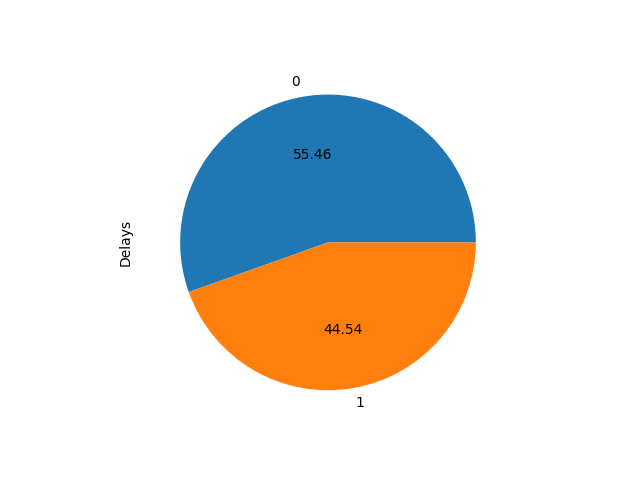
\includegraphics{PieChartDelay}
\caption{Frequenza del Label delay}
 \label{fig:image2}
\end{figure}

Vediamo quindi, che il dataset è sbilanciato; andremo a modificarlo tramite l'utilizzo di oversampling.

\section{Data exploration}
Dopo aver visualizzato graficamente il dataset, andremo a fargli delle modifiche per renderlo più accessibile, e utilizzabile dai modelli di Machine Learning.\\
Prima di tutto rimuoviamo la feature 'id', non utile per il task; andiamo poi a fare l'encoding delle feature categoriche, trasformando le colonne di esse in colonne di interi ordinali, tramite l'utilizzo di OrdinalEncoder. Non ho bisogno di fare label encoding perchè è già corretto così; tramite l'utilizzo dello z-score, andiamo a rimuovere gli outliers (più o meno 9000, quelli con z-score $ > $ 3). Con l'uso di Mutual Information andiamo a verificare la correlazione tra le feature e il label: 

\begin{figure}[H]
\centering
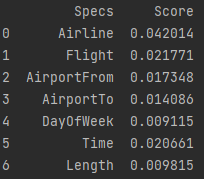
\includegraphics{MutualInformation}
\caption{Risultati MutualInformation con SelectKBest}
 \label{fig:image3}
\end{figure}

\subsection{Feature Selection}
Con la funzione appena usata, andiamo a rimuovere le due feature con score molto basso, DayOfWeek e Length
\subsection{Creazione Test e Training Set}
Andiamo poi a fare lo splitting del Dataset in Training e Test set (rispettivamente 80\% e 20\%); dopo aver fatto ciò è necessario fare oversampling sul training set per bilanciarlo, utilizzando SMOTE
\subsection{Feature Scaling}
Andiamo in fine a fare feature scaling, per aiutare la discesa del gradiente, con l'utilizzo della normalizzazione Min Max (chiaramente con riferimento al training set, ed applicata successivamente al test set)

\section{Comparazione modelli}
Successivamente al preprocessing, è necessario dover scegliere un modello per eseguire il task di classificazione; andrò ad utilizzare i modelli visti a lezione:

\begin{itemize}
\item Logistic Regression \\
\item Decision Tree Classifier \\
\item Random Forest Classifier \\
\item AdaBoost Classifier \\
\item Gradient Boosting Classifier  \\
\item XGB Classifier \\
\end{itemize}

Con l'utilizzo della funzione cross\_val\_score andiamo quindi a provare ogni modello con StratifiedKFoldValidation con K = 10; la funzione ritorna come parametro di comparazione l'accuracy, sarà quindi quella che andremo ad usare.
Ecco i risultati (prima senza rimozione feature, dopo con):
\begin{figure}[H]
  \centering
  \begin{subfigure}[b]{0.6\linewidth}
    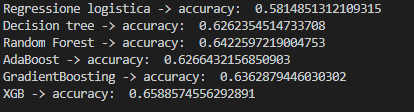
\includegraphics[width=\linewidth]{BeforeRemovingFeatures}
     \caption{Prima di rimuovere DayOfWeek e Length}
  \end{subfigure}
  \begin{subfigure}[b]{0.6\linewidth}
    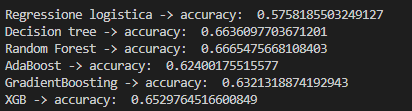
\includegraphics[width=\linewidth]{AfterRemovingFeatures}
    \caption{Dopo averli rimossi}
  \end{subfigure}
  \caption{Risultati Valutazione}
  \label{fig:image4}
\end{figure}

Il modello utilizzato sarà quindi RandomForestClassifier.

\section{Random Forest Classifier}
\subsection{Fine Tuning}
Per andare a fare Fine Tuning degli hyperparametri di Random Forest andremo a usare per prima cosa una funzione di Random Search con RandomizedSearchCV, e poi GridSearch sui parametri nel range dei parametri trovati da Random Search, con l'uso di GridSearchCV.
Purtroppo l'operazione di Grid Search fatta bene è troppo onerosa per la mia postazione, ma il codice è pronto per eseguirla. 
\begin{figure}[H]
 \centering
  \begin{subfigure}[b]{1.3\linewidth}
    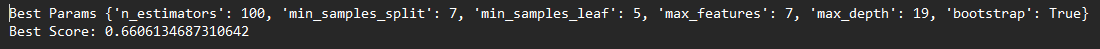
\includegraphics[width=\linewidth]{RandomSearchResults}
     \caption{Risultati RandomSearch}
  \end{subfigure}
  \caption{}
  \label{fig:image5}
\end{figure}
\subsection{Testing Phase}
Andiamo quindi a testare il modello con i parametri ottenuti, ecco di seguito i risultati:
\begin{figure}[H]
 \centering
  \begin{subfigure}[b]{0.7\linewidth}
    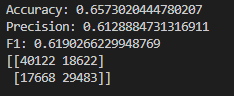
\includegraphics[width=\linewidth]{TestScores}
     \caption{}
  \end{subfigure}
  \begin{subfigure}[b]{0.7\linewidth}
    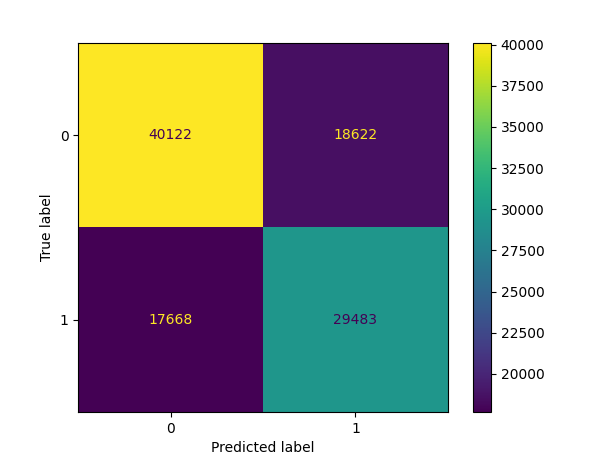
\includegraphics[width=\linewidth]{ConfusionMatrix}
     \caption{}
  \end{subfigure}
  \caption{Risultati}
  \label{fig:image6}
\end{figure}

Con un GridSearch più approfondito probabilmente i risultati sarebbero migliorati.

\section{Artificial Neural Network}
Visto che a lezione abbiamo introdotto le reti neurali, ho deciso di creare un piccolo modello, per fare la stessa task di classificazione sullo stesso dataset (già preprocessato), con l'uso di Keras.
\subsection{Fine Tuning}
Anche qui andremo a fare Fine Tuning, facendo RandomSearch e GridSearch, con l'ausilio di scikeras, libreria che permette di usare gli strumenti di sklearn con Keras.
Ecco i risultati del RandomizedSearch:
\begin{figure}[H]
 \centering
  \begin{subfigure}[b]{0.9\linewidth}
    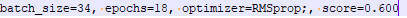
\includegraphics[width=\linewidth]{RandomSearchKeras}
     \caption{Risultati RandomSearch}
  \end{subfigure}
  \caption{}
  \label{fig:image7}
\end{figure}
\subsection{Testing phase}
Vado infine a testare la rete con i parametri trovati:
\begin{figure}[H]
 \centering
  \begin{subfigure}[b]{0.9\linewidth}
    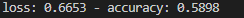
\includegraphics[width=\linewidth]{KerasTest}
     \caption{Risultati RandomSearch}
  \end{subfigure}
  \caption{}
  \label{fig:image8}
\end{figure}
\pagebreak

\section{Conclusioni}
Nonostante un'attenta fase di studio del dataset, e il suo preprocessing, il modello da me scelto e configurato appositamente per l'utlizzo, da dei risultati che non mi soddisfano pienamente: probabilmente la non esecuzione del Grid Search e il basso score di Mutual Information sono alcune delle ragioni del risultato. 



 











\end{document}